\begin{exercice}[Renard rusé]
Un poulailler grillagé de forme rectangulaire mesure 10 mètres de long et 6 mètres de large. Médor, le premier chien de garde, est attaché à un piquet à l'angle du poulailler avec une chaîne de 15 mètres. Il doit surveiller le grillage mais ne peut pas rentrer dans l'enclos. 
\begin{enumerate}
 \item Dessine le poulailler, en précisant l'échelle appropriée que tu auras choisie, puis colorie en rouge la zone protégée par Médor. Repasse en noir la partie du grillage que le renard pourrait attaquer sans danger.
 \item Barbac, le second chien de garde est attaché avec une chaîne de 10 mètres, à l'angle du poulailler le plus proche de celui de Médor.
 
Sur le même schéma, colorie en bleu la zone protégée par Barbac. Le renard peut-il encore attaquer le grillage du poulailler en toute sécurité ?
 \end{enumerate}
\end{exercice}


\begin{exercice}[Agrandissement]
Reproduis la figure en doublant ses dimensions.
\begin{center} 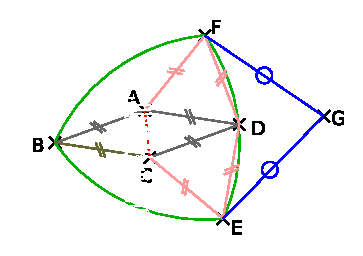
\includegraphics[width=5cm]{agrandissement} \end{center}
\end{exercice}


\begin{exercice}[Construction de l'hexagone]

\vspace{1em}

\begin{minipage}[c]{0.50\linewidth}
Observe attentivement le codage de la figure ci‑contre. 

Déduis-en une méthode pour construire un hexagone régulier de 4 cm de côté puis effectue la construction sur ton cahier.
 \end{minipage} \hfill%
 \begin{minipage}[c]{0.46\linewidth}
  \begin{center} 
\includegraphics[width=3.5cm]{hexagone} \end{center}
  \end{minipage} \\
\end{exercice}


\begin{exercice}[Quadrilatères inscrits dans un cercle]
\begin{enumerate}
 \item Trace un cercle de centre $O$ et de rayon 5 cm. Trace deux diamètres perpendiculaires qui coupent le cercle en quatre points formant le quadrilatère $RIEN$. Quelle est sa nature ?
 \item Construis les médiatrices de $[NO]$ et de $[OI]$. Elles coupent le cercle en quatre points formant le quadrilatère $TOUS$. Quelle est sa nature ?
 \item Les médiatrices coupent $[NI]$ en deux points $M$ et $A$. Quelle est la nature de $ARME$ ?
 \end{enumerate}
\end{exercice}


\begin{exercice}[Élève absent]
Tu étais absent au dernier cours de mathématiques. Marcel et Célestine se sont partagé le travail pour décrire à leur manière les figures. Reproduis-les proprement sur ton cahier :
\begin{enumerate}
 \item Marcel te donne le croquis de la première figure intitulée « les lunules d'Hippocrate ».
 \begin{center} 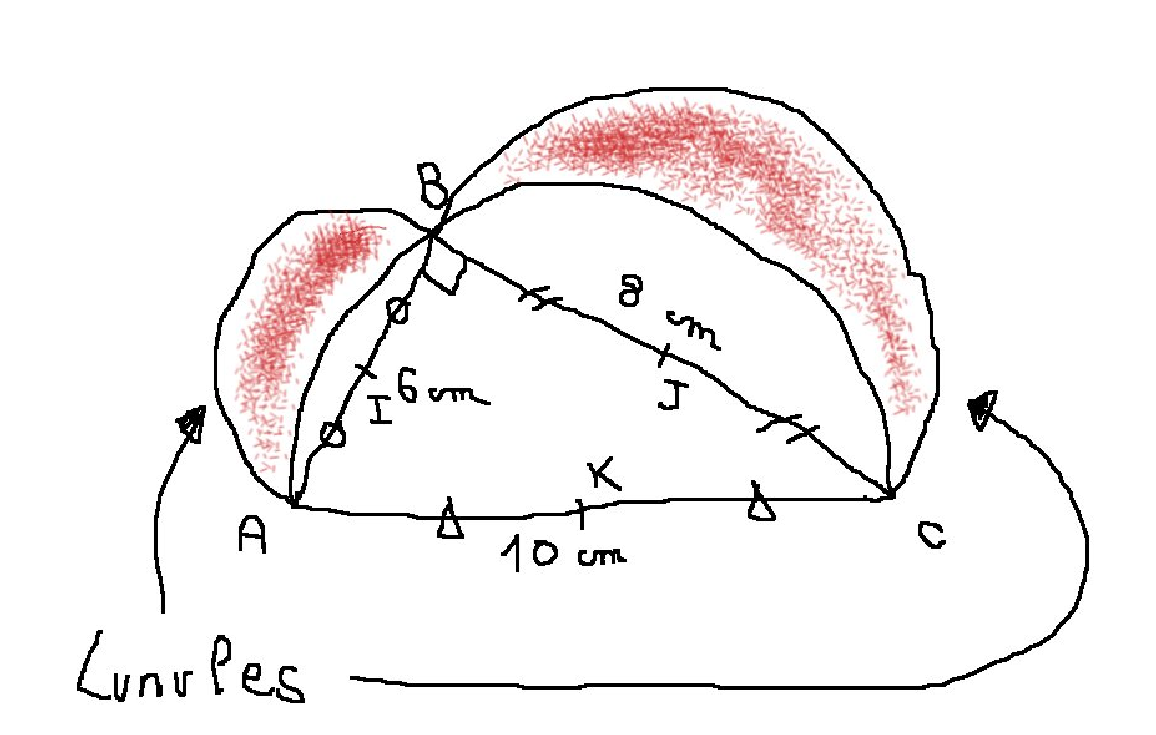
\includegraphics[width=6.8cm]{lunules} \end{center}
 \item Célestine te donne un programme de construction d'un carré $ABCD$ à la règle et au compas :
 
« D'abord, tu traces deux points $A$ et $B$, et la droite $(AB)$.

Pour tracer la droite perpendiculaire à $(AB)$ passant par $A$, tu fais comme cela :
 \begin{itemize}
  \item Place un point $K$ de manière à ce que $A$ soit le milieu de $[KB]$ ;
  \item Trouve un point $L$, équidistant de $K$ et de $B$, autre que le milieu $A$ ;
  \item Trace la droite $(AL)$.
  \end{itemize}
Ensuite, tu fais de la même manière pour tracer la perpendiculaire à $(AB)$ passant par $B$.
  
Enfin, comme tu sais que les côtés d'un carré ont tous la même longueur, tu trouves les points $C$ et $D$.

Et puis pour finir, tu traces joliment ton carré au stylo … »

 \end{enumerate}
\end{exercice}


%%%%%%%%%%%%%%%%%%%%%%%%%%Mise en page

\vspace*{1cm}

\phantom{Pour sauter une ligne}

\newpage
%%%%%%%%%%%%%%%%%%%%%%%%%%%%%%%%%%%%%%




\begin{exercice}[Un intrus]
Construis les figures données par les trois programmes. Quelle est la figure différente des deux autres ?

\begin{enumerate}
 \item \textbf{Programme 1}
 
Trace un cercle de diamètre $[CD]$, de centre $O$ et de rayon 3 cm ;

Place le point $B$ tel que $C$ soit le milieu de $[BO]$ ;

Construis le triangle $ABC$ tel que $AB = 4$ cm et $AC = 5$ cm ;

Trace le segment $[AD]$ ;

Trace les cercles de diamètre $[AD]$ et $[AC]$.

 \item \textbf{Programme 2}
 
Trace un segment $[AC]$ de longueur 5 cm, puis trace le cercle de diamètre $[AC]$ ;

Place un point $B$ sur ce cercle à 4 cm du point $A$ et trace les segments $[AB]$ et $[BC]$ ;

Place les points $O$ et $D$ de manière à ce que les points $B$, $C$, $O$ et $D$ soient alignés dans cet ordre et régulièrement espacés ;

Trace le segment $[AD]$, le cercle de diamètre $[AD]$ et le cercle de centre $O$ passant par $D$.
 \item \textbf{Programme 3}
 
Trace un segment $[AD]$ de longueur 13 cm, et le cercle de diamètre $[AD]$ ;

Place un point $B$ sur le cercle précédent et à 5 cm de $A$ ;

Trace le segment $[BD]$ ;

Place le point $O$ sur le segment $[BD]$ à 4 cm du point $D$ ;

Trace le cercle de centre $O$ passant par $D$, il coupe le segment $[BD]$ en $C$ ;

Trace le segment $[AC]$ ;

Trace le cercle de diamètre $[AC]$.
 \end{enumerate}
\end{exercice}
